%!TEX root =  ./JanasJanssenCuffaro-August2019.tex

%SUBSECTION 3.2
%\subsection{Designing raffles to simulate the quantum correlations} \label{2.2}

We will now design raffles to simulate the quantum correlations found in measurements on the singlet state of two particles with spin $s \ge \sfrac12$ that we investigated in Section \ref{2.1}. In Section \ref{2.2.1}, to set the stage and fix notation, we give a more formal analysis of the raffles for the spin-$\frac12$ case we introduced in Section \ref{1.4}. In Sections \ref{2.2.2}--{2.2.4} we gradually work our way up to higher-spin cases. 

%SUBSUBSECTION 3.2.1
\subsubsection{Spin-$\frac12$}  \label{2.2.1}

The raffles we considered in Section \ref{1.4} all involved baskets containing a mixture of the four ticket types shown in Figure \ref{raffle-tickets-3set2out-i-thru-iv-row} (see the tree structure in Figure \ref{raffle-tickets-3set2out-i-thru-iv} for their numbering). Let $f^{\mathrm{k}}$ denote the fraction of tickets of type $(\mathrm{k})$ in such a basket (with $\mathrm{k} = \mathrm{i}, \mathrm{ii}, \mathrm{iii}, \mathrm{iv}$). These ticket fractions evidently are non-negative and normalized:
\begin{equation}
f^{\mathrm{k}}\geq 0 \; (\mathrm{k} = \mathrm{i}, \mathrm{ii}, \mathrm{iii}, \mathrm{iv}) \quad\text{and}\quad \sum_{\mathrm{k=i}}^{\mathrm{iv}} f^{\mathrm{k}}=1.
  \label{3-simplex}
\end{equation}

\begin{figure}[ht]
 \centering
   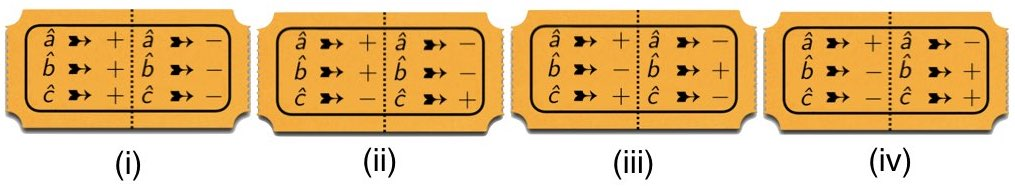
\includegraphics[width=4.5in]{raffle-tickets-3set2out-i-thru-iv-row.jpeg} 
   \caption{The four different raffle tickets for three settings and two outcomes (cf.\ Figure \ref{raffle-tickets-3set2out-i-thru-iv}).}
   \label{raffle-tickets-3set2out-i-thru-iv-row}
   \end{figure}
   
As we observed in Section \ref{1.4} (see note \ref{dense}), the imagery of a basket with a mix of tickets restricts us to values for $f^{\mathrm{k}}$ that are rational numbers. We will continue to discuss our raffles in terms of baskets of tickets, but we do want to point out that with a simple change of imagery we can accommodate real values as well. Instead of  baskets with tickets, consider wheels of fortune such as those shown in Figure \ref{wheelsoffortune}. These wheels have pie charts printed on them showing the mix of tickets in a particular raffle, each ticket of type $(\mathrm{k})$ occurring with a fraction $f^{\mathrm{k}}$ in the raffle corresponding to a segment $f^{\mathrm{k}} \times 100\%$ of the pie chart. Instead of randomly drawing a ticket from a basket, we would spin the wheel of fortune and pick a ticket of the type the pointer points to when the wheel of fortune comes to rest.   
          
\begin{figure}[ht]
 \centering
   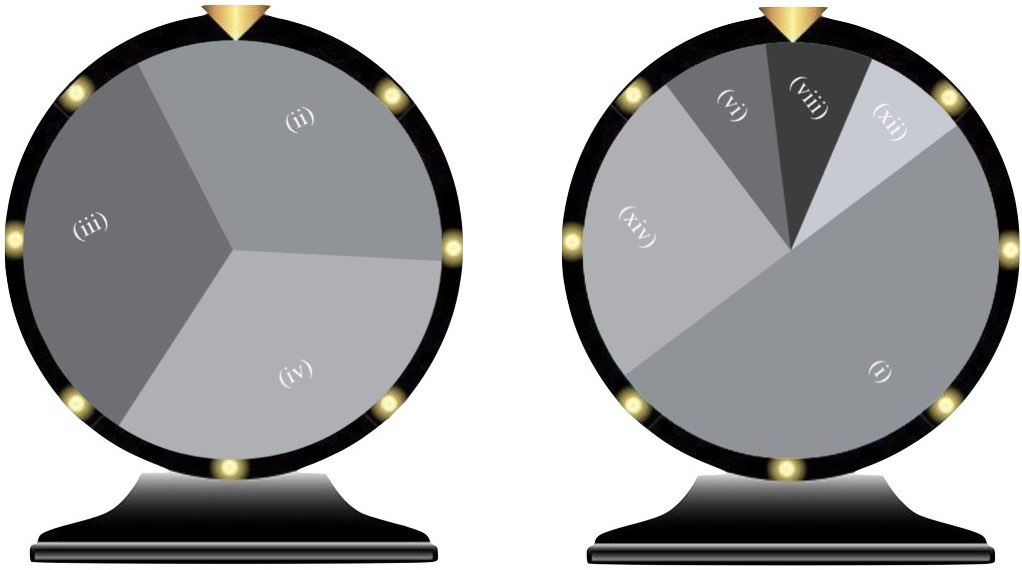
\includegraphics[width=4.5in]{wheelsoffortune.jpeg} 
   \caption{Wheels of fortune for two raffles. The one on the left is for a raffle with a mix of $\sfrac13$ each of tickets of type (ii), (iii) and (iv) in Figure \ref{raffle-tickets-3set2out-i-thru-iv-row}. This is raffle (b) in Figure \ref{CA-3set2out-raffle-mix} in Section \ref{1.4}, our optimal simulation of the Mermin correlation array in Figure \ref{CA-3set2out-Mermin}. The one on the right is for a 75\%/25\% mix of the admissible raffles ($\alpha$) and ($\beta$) in Figure \ref{admissible-raffles-spin1} in Section \ref{2.2.2}.}
   \label{wheelsoffortune}
   \end{figure}  
%Pie charts for wheels of fortune for two raffles. The pie chart on the left is for a raffle with a mix of $\sfrac13$ each of tickets of type (ii), (iii) and (iv) in Figure \ref{raffle-tickets-3set2out-i-thru-iv-row}. This is raffle (b) in Figure \ref{CA-3set2out-raffle-mix} in Section \ref{1.4}, our optimal simulation of the Mermin correlation array in Figure \ref{CA-3set2out-Mermin}. The pie chart on the right is for a 75\%/25\% mix of the admissible raffles ($\alpha$) and ($\beta$) in Figure \ref{admissible-raffles-spin1} in Section \ref{2.2.2}. 

When we think of 
\begin{equation}
\vec{f}\equiv (f^{\mathrm{i}},f^{\mathrm{ii}},f^{\mathrm{iii}},f^{\mathrm{iv}})
\label{raffle point f}
\end{equation}
as a point in $\mathbb{R}^{4}$, the constraints in Eq.\ (\ref{3-simplex}) define what is conventionally known as the \emph{3D standard simplex} or \emph{3-simplex} in $\mathbb{R}^{4}$.  Equivalently, this simplex is the convex hull of the four points 
\begin{equation}
\vec{f}_{\mathrm{i}}= 
\begin{pmatrix}
1 \\
0 \\
0 \\
0
\end{pmatrix}, \quad 
\vec{f}_{\mathrm{ii}} = \begin{pmatrix}
0 \\
1 \\
0 \\
0
\end{pmatrix}, \quad
\vec{f}_{\mathrm{iii}} = \begin{pmatrix}
0 \\
0 \\
1 \\
0
\end{pmatrix}, \quad 
\vec{f}_{\mathrm{iv}} = \begin{pmatrix}
0 \\
0 \\
0 \\
1
\end{pmatrix},
\label{single ticket raffles}
\end{equation}
each corresponding to a raffle with just one type of ticket in the basket. These single-ticket raffles are \emph{basic} in the sense that any raffle can be obtained as a mix of them. As the notation already suggests, Eq.\ (\ref{single ticket raffles}) can also be seen as giving the unit vectors of an \emph{orthonormal basis} in which we can expand vectors characterizing arbitrary raffles. The quantity $\vec{f}$ in Eq.\ (\ref{raffle point f}) can then be thought of as the vector
\begin{equation}
\vec{f} =  \sum_{\mathrm{k=i}}^{\mathrm{iv}} f^{\mathrm{k}} \vec{f}_{\mathrm{k}}
\label{expansion of vec f} 
\end{equation}
and the ticket fractions $f^{\mathrm k}$ as its components in this basis.

The 3-simplex is a polytope in 4D Euclidean space and as such cannot be visualized. To circumvent this problem we consider triplets of anti-correlation coefficients rather than quartets of ticket fractions. The anti-correlation coefficient $\chi_{ab}|_{\vec{f}}$ for an arbitrary (mixed or single-ticket) raffle characterized by some vector $\vec{f}$ is defined as (cf.\ Eq.\ (\ref{chi as corr coef}) in Section \ref{1.3}):
\begin{equation}
 \chi_{ab} |_{\vec{f}} \equiv \left. -\frac{\langle X^A_a X^B_b \rangle}{\sigma^A_a \sigma^B_b} \right|_{\vec{f}}.
 \label{chi for f spin 1/2} 
\end{equation}
This anti-correlation coefficient is equal to the weighted average of those for the four single-ticket raffles in Eq.\ (\ref{single ticket raffles}) with the weights given by the ticket fractions $f^{\mathrm{k}}$. In Section \ref{1.4}, we already used this property of our raffles. We will now give a formal proof of it. 
%The result for the spin-$\frac12$ case can easily be generalized to higher-spin cases.
%some wrinkles we will encounter when dealing with raffles for higher-spin cases.  

We start by evaluating the covariance in the numerator on the right-hand side of Eq.\ (\ref{chi for f spin 1/2}) (cf.\ Eq.\ (\ref{prob 2 exp})). By definition,
\begin{equation}
\langle X^A_a X^B_b \rangle \big|_{\vec{f}\,} = \!\! \sum_{m_1, m_2} \! m_1  m_2 \, \mathrm{Pr}(m_1 m_2| \hat{a} \,\hat{b}) \Big|_{\vec{f}} \;, 
 \label{chi for f spin 1/2 a}
\end{equation}
where the outcomes $m_1$ and $m_2$ can only take on the values $\pm \sfrac12$ (if we set $\bbar$ and $\hbar$ equal to 1). It immediately follows from the design of our raffles that the probability of finding some combination of outcomes for some combination of settings in a raffle with a mix of tickets characterized by $\vec{f}$ is the weighted average of those same probabilities in the four basic single-ticket raffles with the weights given by the ticket fractions:
\begin{equation}
\mathrm{Pr}(m_1 m_2| \hat{a} \,\hat{b}) \big|_{\vec{f}\,} = \sum_{\mathrm{k} = \mathrm{i}}^{\mathrm{iv}} f^{\mathrm{k}} \, \mathrm{Pr}(m_1 m_2| \hat{a} \,\hat{b}) 
\Big|_{\vec{f}_{\mathrm{k}}}.
\label{chi for f spin 1/2 b}
\end{equation}
The probabilities on the right-hand side take on a very simple form: they are $\sfrac12$ if the ticket has the combination of outcomes $(X_a = m_1, X_b = m_2)$ and zero if it does not. For example, the tickets in Figure \ref{raffle-tickets-3set2out-i-thru-iv-row} tell us that 
\begin{equation}
\begin{array}{c}
 \mathrm{Pr}\!\left({\textstyle \frac12}, -{\textstyle \frac12} \Big| \hat{a} \,\hat{b}\right) \Big|_{\vec{f}_{\mathrm{i}}} 
 = \mathrm{Pr}\!\left({\textstyle \frac12}, -{\textstyle \frac12} \Big| \hat{a} \,\hat{b}\right) \Big|_{\vec{f}_{\mathrm{ii}}} \! = {\displaystyle{\frac12}}, \\[.6cm]
\mathrm{Pr}\!\left({\textstyle \frac12}, -{\textstyle \frac12} \Big| \hat{a} \,\hat{b}\right) \Big|_{\vec{f}_{\mathrm{iii}}} 
\!\! = \mathrm{Pr}\!\left({\textstyle \frac12}, -{\textstyle \frac12} \Big| \hat{a} \,\hat{b}\right) \Big|_{\vec{f}_{\mathrm{iv}}} \!\! = 0. 
\end{array}
\label{chi for f spin 1/2 ba}
\end{equation}
For this combination of outcomes, Eq.\ (\ref{chi for f spin 1/2 b}) thus gives
\begin{equation}
\mathrm{Pr}\!\left({\textstyle \frac12}, -{\textstyle \frac12} \Big| \hat{a} \,\hat{b}\right) \Big|_{\vec{f}} = \frac12 \big( f^{\mathrm{i}} + f^{\mathrm{ii}} \big).
\end{equation}
As this example illustrates, Eq.\ (\ref{chi for f spin 1/2 b}) is a more formal expression of another feature of our raffles we repeatedly made use of in Section \ref{1.4}: the entries in the correlation array for a mixed raffle are weighted averages of the corresponding entries in the correlation arrays for single-ticket raffles. 

Inserting Eq.\ (\ref{chi for f spin 1/2 b}) into Eq.\ (\ref{chi for f spin 1/2 a}) and changing the order of the summations, we see that the covariance $\langle X^A_a X^B_b \rangle$ in a mixed raffle is likewise the weighted average of that same covariance in the four single-ticket raffles:
\begin{equation}
\langle X^A_a X^B_b \rangle \big|_{\vec{f}} = \sum_{\mathrm{k} = \mathrm{i}}^{\mathrm{iv}} f^{\mathrm{k}} \sum_{m_1, m_2} \! m_1  m_2 \, \mathrm{Pr}(m_1 m_2| \hat{a} \,\hat{b}) 
\Big|_{\vec{f}_{\mathrm{k}}} =  \sum_{\mathrm{k} = \mathrm{i}}^{\mathrm{iv}} f^{\mathrm{k}} \langle X^A_a X^B_b \rangle \big|_{\vec{f}_{\mathrm{k}}}. 
\label{chi for f spin 1/2 c}
\end{equation}

Because the diagonal cells in the correlation arrays for raffles with any mix of tickets of types (i) through (iv) in Figure \ref{raffle-tickets-3set2out-i-thru-iv-row} are the same, the standard deviations in the expression on the right-hand side of Eq.\ (\ref{chi for f spin 1/2 a}) are also the same for all these raffles. For any $\vec{f}$, they are given by Eq.\ (\ref{SD for adm raffle 2}) in Section \ref{1.6} for $s=\sfrac12$:
\begin{equation}
\sigma_a  \big|_{\vec{f}} = \sigma_b  \big|_{\vec{f}} = \sigma_{s = \sfrac12} = \sqrt{\frac{s(s+1)}{3}} = \frac12.
\label{chi for f spin 1/2 d}
\end{equation}

Substituting Eq.\ (\ref{chi for f spin 1/2 c}) into Eq.\ (\ref{chi for f spin 1/2}) and using Eq.\ (\ref{chi for f spin 1/2 d}), we arrive at
\begin{equation}
\chi_{ab} |_{\vec{f}} = -\frac{\langle X^A_a X^B_b \rangle \big|_{\vec{f}}}{\sigma_{s=\sfrac12}^2}  =
\sum_{\mathrm{k} = \mathrm{i}}^{\mathrm{iv}} f^{\mathrm{k}} \left( \! \left. -\frac{\langle X^A_a X^B_b \rangle  }{ \sigma_a \sigma_b }  \right|_{ \vec{f}_{ \mathrm{k} } } \right)
=  \sum_{\mathrm{k} = \mathrm{i}}^{\mathrm{iv}} f^{\mathrm{k}} \, \chi_{ab} |_{\vec{f}_{\mathrm{k}} },
\label{chi for f spin 1/2 e}
\end{equation}
which is what we set out to prove. 

Similar relations hold for $\chi_{ac}$ and $\chi_{bc}$. We combine these three relations and write them in matrix form: 
\begin{equation}
\left. \begin{pmatrix}
\chi_{ab}\\[.2cm]
\chi_{ac}\\[.2cm]
\chi_{bc}
\end{pmatrix} \right|_{\vec{f}} = 
\begin{pmatrix}
   \chi_{ab} |_{\vec{f}_{\mathrm{i}} } \; & \; \chi_{ab} |_{\vec{f}_{\mathrm{ii}} } \; & \; \chi_{ab} |_{\vec{f}_{\mathrm{iii}} } \; & \; \chi_{ab} |_{\vec{f}_{\mathrm{iv}} } \\[.4cm]
     \chi_{ac} |_{\vec{f}_{\mathrm{i}} } & \chi_{ac} |_{\vec{f}_{\mathrm{ii}} } & \chi_{ac} |_{\vec{f}_{\mathrm{iii}} } & \chi_{ac} |_{\vec{f}_{\mathrm{iv}} }  \\[.4cm]
     \chi_{bc} |_{\vec{f}_{\mathrm{i}} } & \chi_{bc} |_{\vec{f}_{\mathrm{ii}} } & \chi_{bc} |_{\vec{f}_{\mathrm{iii}} } & \chi_{bc} |_{\vec{f}_{\mathrm{iv}} }  
\end{pmatrix}
\begin{pmatrix} f^{\mathrm{i}} \\[.2cm]
f^{\mathrm{ii}} \\[.2cm]
f^{\mathrm{iii}} \\[.2cm]
f^{\mathrm{iv}} \end{pmatrix}.
\label{Mapping spin 1/2}
\end{equation}
The $3 \times 4$ matrix $M$ on the right-hand side thus serves as a map from the 3-simplex of possible ticket fractions to the \emph{anti-correlation polyhedron} (see the introduction of Section \ref{2} for a definition). Denoting the vector on the left-hand side as $\vec{\chi}|_{\vec{f}}$, we can write Eq.\ (\ref{Mapping spin 1/2}) more compactly as
\begin{equation}
\vec{\chi}|_{\vec{f}} \equiv M \vec{f}.
\label{Mapping spin 1/2 a}
\end{equation}
The matrix elements of $M$ can be read off of Table \ref{values of chi} in Section \ref{1.4} (or directly from the tickets in Figure \ref{raffle-tickets-3set2out-i-thru-iv-row}: note that $1/\sigma_{s=\sfrac12}^2 = 4$ cancels the 4 in the denominators of the covariances):
\begin{equation}
M = \begin{pmatrix}
    M_{ab}^{\mathrm{i}} & M_{ab}^{\mathrm{ii}} & M_{ab}^{\mathrm{iii}} & M_{ab}^{\mathrm{iv}} \\[.2cm]
    M_{ac}^{\mathrm{i}} & M_{ac}^{\mathrm{ii}} & M_{ac}^{\mathrm{iii}} & M_{ac}^{\mathrm{iv}} \\[.2cm] 
    M_{bc}^{\mathrm{i}} & M_{bc}^{\mathrm{ii}} & M_{bc}^{\mathrm{iii}} & M_{bc}^{\mathrm{iv}}
\end{pmatrix}
= \begin{pmatrix}
    1 & 1 & -1 & -1 \\[.2cm]
    1 & -1 & 1 & -1 \\[.2cm]
    1 & -1 & -1 & 1 
\end{pmatrix}.
\label{Mapping spin 1/2 b}
\end{equation}
$M$ will map the basis vectors in Eq.\ (\ref{single ticket raffles}) for the four single-ticket raffles onto vectors whose components are the columns of $M$:
\begin{equation}
\vec{\chi}|_{\vec{f}_{\mathrm{i}}} = 
\begin{pmatrix}
1 \\
1 \\
1
\end{pmatrix},
\;\;
\vec{\chi}|_{\vec{f}_{\mathrm{ii}}} = 
\begin{pmatrix}
1 \\
-1 \\
-1
\end{pmatrix},
\;\;
\vec{\chi}|_{\vec{f}_{\mathrm{iii}}} =
\begin{pmatrix}
-1 \\
1 \\
-1
\end{pmatrix},
\;\;
\vec{\chi}|_{\vec{f}_{\mathrm{iv}}} = 
\begin{pmatrix}
-1 \\
-1 \\
1
\end{pmatrix}.
\label{Mapping spin 1/2 c}
\end{equation}
These vectors correspond to the vertices (i) through (iv) of the tetrahedron we found in Section \ref{1.4} (see Figure \ref{tetrahedron}). 


%SUBSUBSECTION 3.2.2
\subsubsection{Spin-1}  \label{2.2.2}

Having reviewed the case of spin-$\frac12$, we now move to new territory and consider the case of spin-$1$. The first change is to the number of tickets. There are now three possible outcomes for the three settings: $1$, $0$ and $-1$ (again setting $\hbar = \bbar =1$). This means that there are now $3^3=27$ ways to specify the outcomes on one side of the ticket, which, as before, determine the outcomes on the other side. Since it is totally random which side of the ticket goes to Alice and which side goes to Bob, it suffices to consider the 14 ticket types labeled $(\mathrm{i})$ through $(\mathrm{xiv})$ shown in Figure \ref{raffle-tickets-3set3out-i-xiv} (to number these we used a tree structure similar to the one in Figure \ref{raffle-tickets-3set2out-i-thru-iv}). 

\begin{figure}[h!]
 \centering
   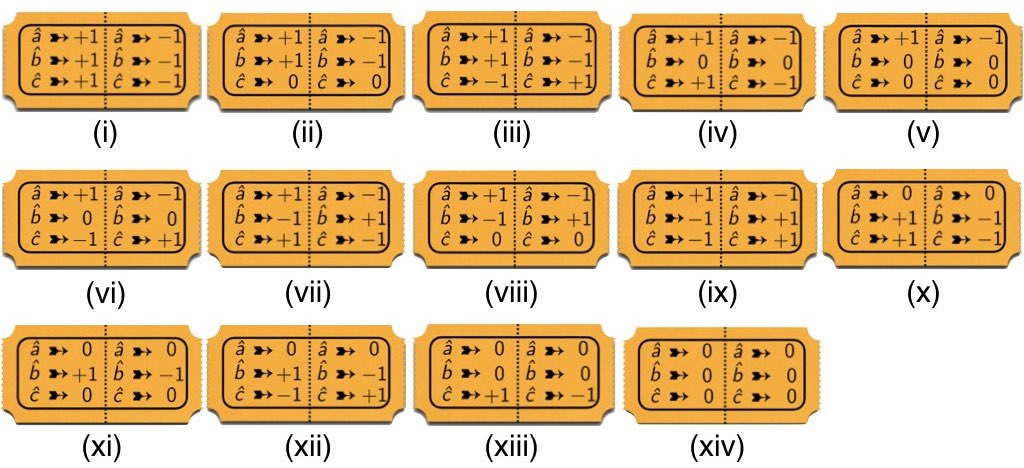
\includegraphics[width=4.5in]{raffle-tickets-3set3out-i-xiv.jpeg} 
   \caption{The fourteen different types of raffle tickets for three settings and three outcomes that are left once the condition is imposed that, when Alice and Bob use the same setting, they should find opposite results if the outcome is $+1$ or $-1$ but the same result if the outcome is $0$.}
   \label{raffle-tickets-3set3out-i-xiv}
\end{figure}

A generic raffle is some mix of these 14 ticket types. Geometrically this corresponds to a point in the 13D simplex, defined as the convex hull of the 14 points corresponding to the standard unit basis vectors in $\mathbb{R}^{14}$ (cf.\ Eqs.\ (\ref{3-simplex})--(\ref{expansion of vec f}), with the index k now running from i to xiv). The diagram in Figure \ref{flowchart} provides a flow chart for how to get from this simplex in $\mathbb{R}^{14}$ to a polyhedron in $\mathbb{R}^3$ characterizing the class of quantum correlations found in measurements on the singlet state of two spin-1 particles that can be simulated---albeit, as we will see, imperfectly---with these raffles. 

\begin{figure}[ht]
 \centering
   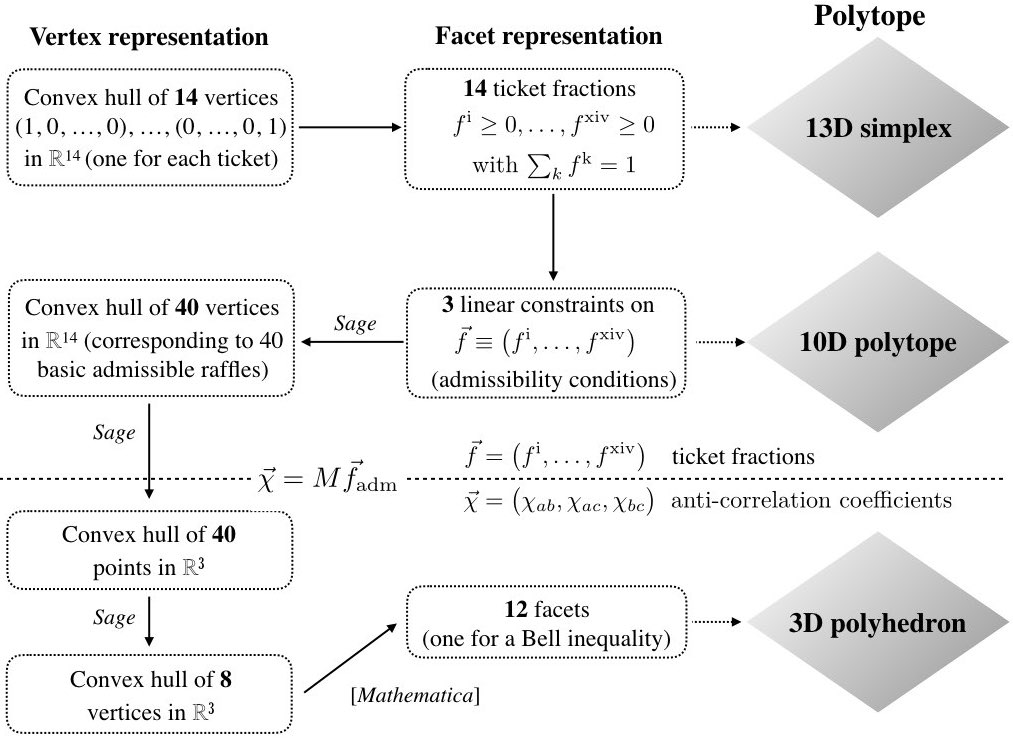
\includegraphics[width=4.5in]{flowchart.jpeg} 
   \caption{Flow chart illustrating the construction of the polyhedron characterizing the set of correlations that (a) can be generated with raffles mixing tickets of types (i) through (xiv) in Figure \ref{raffle-tickets-3set3out-i-xiv} and (b) replicate key features of the quantum correlations for measurements on the singlet state of two spin-1 particles.}
   \label{flowchart}
   \end{figure}

A polytope can be represented either in terms of its vertices or in terms of its facets. These are called the \emph{V-representation} and the \emph{H-representation}, respectively. The $H$-representation is given in terms of a set of inequalities restricting points to be on one side of some (hyper-)plane (hence the ``$H$'', which stands for ``half-space"). As our flow chart illustrates, we switch back and forth between these two representations as we go from the 13D simplex to the 3D polyhedron. For several computation-intensive
steps we used the open-source mathematical software system SageMath. 

The tickets for the spin-1 case immediately reveal one key difference with the spin-$\frac12$ case that we already drew attention to in Section \ref{1.6}. Our raffle tickets can only have two outcomes for each setting. As soon as there are more than two possible outcomes (and for spin $s$ there are $2s + 1$), it is thus impossible for all outcomes to occur in equal proportion in a single-ticket raffle. Yet this is what Alice and Bob find if they use the same setting in the quantum experiment these raffles are supposed to simulate. In terms of probabilities, the problem is that for spins greater than $\sfrac12$, single-ticket raffles---while non-signaling by construction---do not give uniform marginals, whereas measurements on two particles of arbitrary spin entangled in the singlet state do (as we showed in Section \ref{2.1.4}). The correlation array in Figure \ref{CA-3set3out-raffle-vi} for a single-ticket raffle illustrates the problem. The array is non-signaling but the marginals take on three different values: $0$, $\sfrac12$ and $1$. The solution to this problem is to allow only mixed raffles that give uniform marginals. 

\begin{figure}[ht]
 \centering
   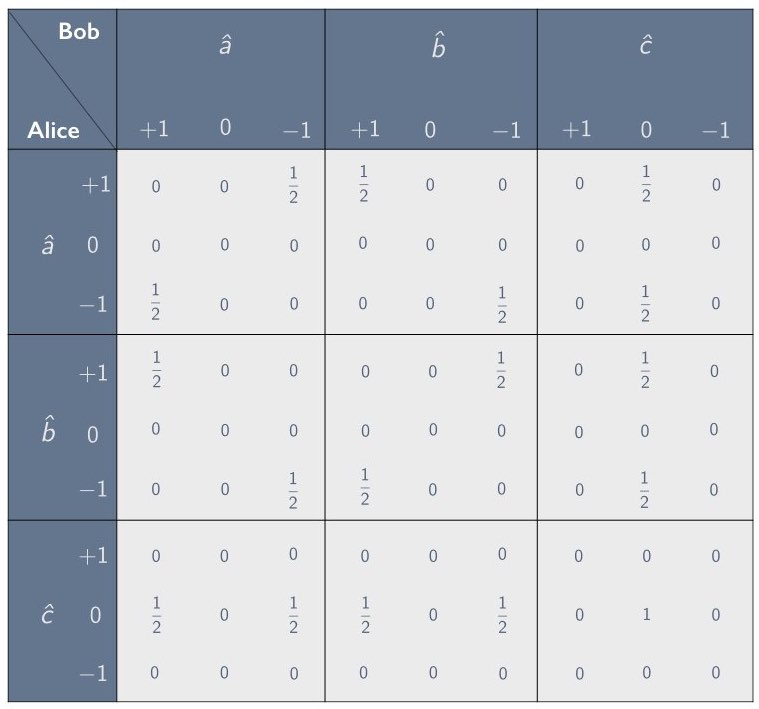
\includegraphics[width=4in]{CA-3set3out-raffle-vi.jpeg} 
   \caption{Correlation array for a single-ticket raffle with tickets of type (vi) (see Figure \ref{raffle-tickets-3set3out-i-xiv}).}
   \label{CA-3set3out-raffle-vi}
\end{figure}

\begin{figure}[ht]
 \centering
   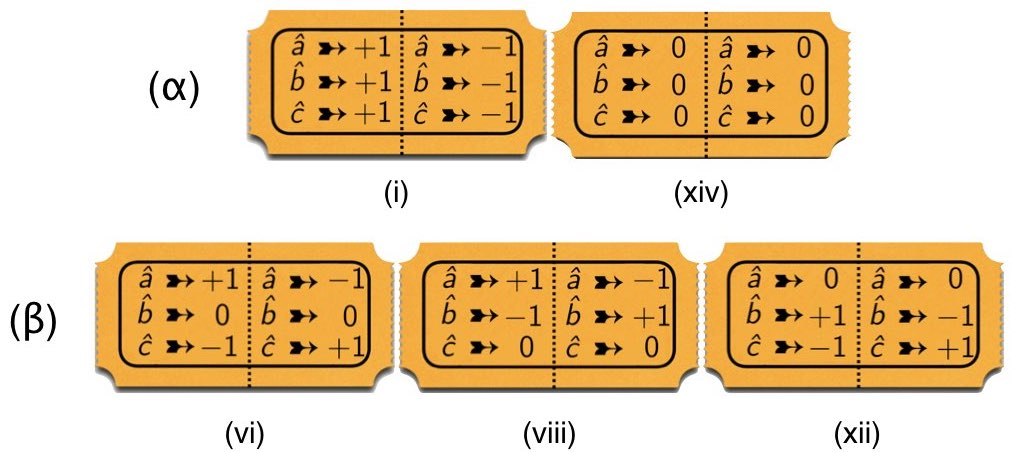
\includegraphics[width=4.5in]{admissible-raffles-spin1.jpeg} 
   \caption{Two mixed raffles giving uniform marginals: in ($\alpha$) $\sfrac23$ of the tickets are of type (i) and $\sfrac13$ is of type (xiv); ($\beta$) has $\sfrac13$ each of types (vi), (viii) and (xii).}
   \label{admissible-raffles-spin1}
\end{figure}

Before we show how to construct such admissible raffles, we remind the reader of another property of the correlation array in Figure \ref{CA-3set3out-raffle-vi}: the $9 \times 9$ matrix formed by its entries is symmetric. This is a direct consequence of the design of our raffles (for any number of outcomes per setting). Since the correlation array obviously stays the same if Alice and Bob swap both the ticket stubs they receive and the settings they use, its entries for any one of our raffles satisfy  
\begin{equation}
\mathrm{Pr}\!\left(m_1 m_2 \big| \hat{a} \,\hat{b}\right)
=  \mathrm{Pr}\!\left(m_2 m_1 \big| \hat{b} \,\hat{a}\right).
\label{swap symmetry}
\end{equation}

In our raffles for the spin-$\frac12$ case, it followed directly from the symmetry of the $6 \times 6$ matrix for the correlation array as a whole that the $2 \times 2$ matrices formed by the entries of its individual cells are also symmetric and that cells on opposite sides of the diagonal are the same (see, e.g., Figure \ref{CA-3set2out-raffles-i-thru-iv}). For the correlation arrays for the quantum correlations that we are trying to simulate with our raffles, both claims are true for arbitrary spin $s$ (see Figure \ref{CA-cell-spin1-chi} for spin-1; recall that $\chi_{ab} = \cos{\varphi_{ab}} = \cos{\varphi_{ba}} = \chi_{ba}$). Neither one is true, however, for the cells in the correlation array for the single-ticket raffle in Figure \ref{CA-3set3out-raffle-vi}.  In four of the nine cells, the $3 \times 3$ matrices formed by its entries are not symmetric and the matrices for cells on opposite sides of the diagonal are each other's transpose. 

Fortunately, these discrepancies are easily dealt with. First note that the transpose of a symmetric matrix is that matrix itself. Demanding individual cell symmetry thus suffices to ensure that cells on opposite sides of the diagonal are identical. Second, with raffles for the spin-1 case, as we will see, demanding uniform marginals suffices to ensure cell symmetry. In raffles for higher-spin cases, however, cell symmetry calls for additional admissibility conditions (see Section \ref{2.2.3}).

There is one more difference between the spin-$\frac12$ and the spin-1 case that we want to highlight. In the spin-$\frac12$ case, as we saw in Section \ref{1.4},  the probabilities in a cell of a correlation array are fully determined by the anti-correlation coefficient for that cell. In quantum mechanics, this remains true for spin $s > \sfrac12$ even though the dependence of the probabilities on the anti-correlation coefficient is no longer linear (see, e.g., Figure \ref{CA-cell-spin1-chi} in Section \ref{2.1} for $s=1$). As soon as $s > \sfrac12$, however, it is no longer true for the raffles meant to simulate these quantum correlations. In the spin-1 case, as we will see in Section \ref{2.2.3}, it takes two parameters to fix the entries in any off-diagonal cell of a correlation array for an admissible raffle. In these higher spin cases, the same triplet of anti-correlation coefficients will therefore in general correspond to more than one admissible raffle. This should not surprise us. We should not expect the projection from higher-dimensional polytopes of admissible raffles to anti-correlation polyhedra to be injective.    

We are now ready to start constructing raffles for the spin-1 case that give uniform marginals. Figure \ref{admissible-raffles-spin1} shows two examples of such raffles. The first, labeled ($\alpha$) and characterized by the vector 
\begin{equation}
\vec{f}_\alpha = \frac23 \vec{f}_{\mathrm{i}} + \frac13 \vec{f}_{\mathrm{xiv}},
\label{spin 1 raffle alpha}
\end{equation}
is probably the easiest way to ensure uniform marginals. It uses tickets with the same outcomes for all three settings. With two tickets of type (i) and one of type (xiv), all three outcomes occur six times for all three settings. That means that, for all three settings, all three outcomes will be found with equal probability by both Alice and Bob. In the raffle labeled ($\beta$) and characterized by the vector  
\begin{equation}
\vec{f}_\beta =  \frac13 \left( \vec{f}_{\mathrm{vi}} + \vec{f}_{\mathrm{viii}} + \vec{f}_{\mathrm{xii}}\right),
\label{spin 1 raffle beta}
\end{equation}
the outcomes for setting $\hat{a}$ are the same as those in raffle ($\alpha$) while the outcomes for settings $\hat{b}$ and $\hat{c}$ are permutations of those in raffle ($\alpha$). These permutations were chosen so as to make the sum $X_a + X_b + X_c$ vanish on both sides of all three tickets. As we saw in Section \ref{1.6}, this means that the (anti-)correlations produced by this raffle are represented by a point on the elliptope in Figure \ref{elliptope}. 

\begin{figure}[ht]
 \centering
   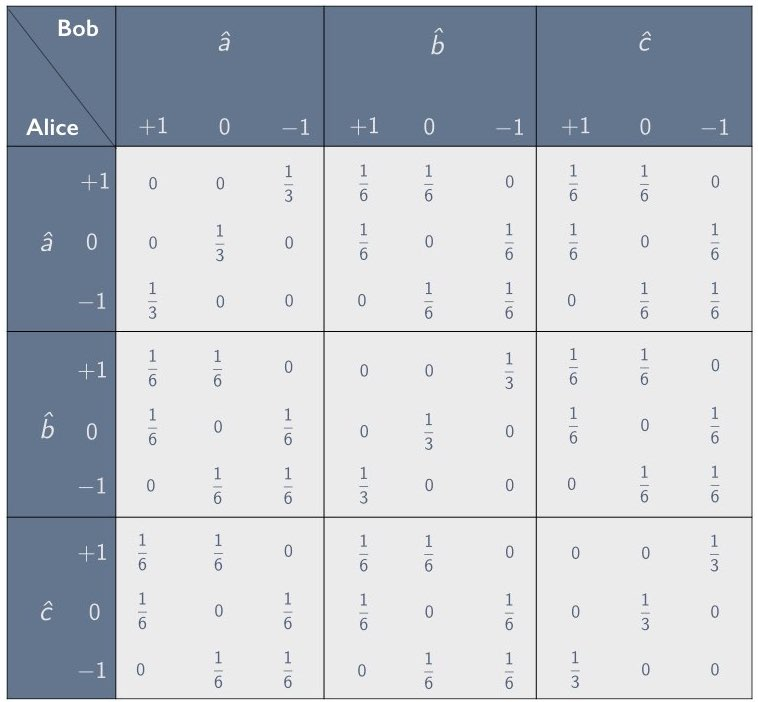
\includegraphics[width=4in]{CA-3set3out-raffle-33vi33viii33xii.jpeg} 
   \caption{Correlation array for a raffle with equal numbers of tickets of types (vii), (viii) and (xii) (see Figure \ref{admissible-raffles-spin1}, ($\beta$)).}
   \label{CA-3set3out-raffle-33vi33viii33xii}
\end{figure}

Figure \ref{CA-3set3out-raffle-33vi33viii33xii} shows the correlation array for the mixed raffle ($\beta$). Unlike the correlation array in Figure \ref{CA-3set3out-raffle-vi} (for a single-ticket raffle), it has uniform marginals, as we demanded. The diagonal cells in correlation arrays for raffles that give uniform marginals are all the same. The standard deviations $\sigma_a$, $\sigma_b$ and $\sigma_c$ for such raffles are equal to $\sigma_{s=1} = \sqrt{\sfrac23}$, in accordance with the general formula $\sigma_s^2 = \frac13 s(s+1)$ (see Eq.\ (\ref{SD for adm raffle 2}) in Section \ref{1.6}). This is not true for single-ticket raffles or raffles with an arbitrary mix of ticket types. This provides another reason for restricting ourselves to raffles that give uniform marginals. The projection from $\mathbb{R}^{14}$ to $\mathbb{R}^3$ we are after only works if we can assume that the diagonal cells of the correlation arrays and thus the standard deviations $\sigma_a$, $\sigma_b$ and $\sigma_c$ are the same for all raffles considered.

With the help of the correlation array in Figure \ref{CA-3set3out-raffle-33vi33viii33xii}, we find that
\begin{equation}
\langle X^A_a X^B_b \rangle \big|_{\vec{f}_\beta} = \mathrm{Pr}(1 1| \hat{a} \,\hat{b}) \Big|_{\vec{f}_\beta} + \mathrm{Pr}(-1 -\!1| \hat{a} \,\hat{b}) \Big|_{\vec{f}_\beta} 
= \frac13
\label{covariance ab raffle beta}
\end{equation}
Inserting Eq.\ (\ref{covariance ab raffle beta}) and $\sigma^A_a \sigma^A_b = \sigma_{s=1}^2 = \sfrac23$ into Eq.\ (\ref{chi for f spin 1/2}), we arrive at 
\begin{equation}
 \chi_{ab} |_{\vec{f}_\beta} = \left. -\frac{\langle X^A_a X^B_b \rangle}{\sigma^A_a \sigma^B_b} \right|_{\vec{f}_\beta} = -\sfrac12.
\end{equation}
We similarly find that $ \chi_{ac} |_{\vec{f}_\beta} =  \chi_{bc} |_{\vec{f}_\beta} = -\sfrac12$. The raffle ($\beta$) is thus represented by the point 
\begin{equation}
\left( \chi_{ab}, \chi_{ac}, \chi_{bc} \right)  \big|_{\vec{f}_\beta} = \left(-\sfrac12, -\sfrac12, -\sfrac12 \right)
\label{raffle beta = -1/2^3}
\end{equation}
on the elliptope, where the sum $\chi_{ab} + \chi_{ac} + \chi_{bc}$ has its absolute minimum value of $-\sfrac32$ (cf.\ Section \ref{1.6}). With raffle ($\beta$) we have thus constructed a toy example of a local hidden-variable theory with which we can reach the Tsirelson bound  for this setup. This raffle, however, still fails to reproduce all features of the correlation array for the corresponding quantum case. 

In quantum mechanics, Eq.\ (\ref{raffle beta = -1/2^3}) holds for the correlations found in measurements on the singlet state of two particles of arbitrary (half-)integer spin $s$ if each of  the angles $\varphi_{ab}$, $\varphi_{ac}$ and $\varphi_{bc}$ between the three measuring directions is equal to $120\degree$. In that case the anti-correlation coefficients $\chi_{ab}$, $\chi_{ac}$ and $\chi_{bc}$ are all equal to $\cos 120\degree = -\sfrac12$. By demanding uniform marginals, we made sure that the diagonal cells of the correlation array for raffle ($\beta$) in Figure \ref{CA-3set3out-raffle-33vi33viii33xii} are the same as those of the quantum correlation array for $s=1$ we are trying to simulate. The six off-diagonal cells, however, while identical to each other, differ from the six identical off-diagonal cells in this quantum correlation array. Below we put the entries of two of these off-diagonal cells side-by-side, for raffle ($\beta$) on the left, for the quantum correlations on the right (we obtain the latter by substituting $\chi_{ab} = -\sfrac12$ in the $\hat{a} \hat{b}$ cell in Figure \ref{CA-cell-spin1-chi} in Section \ref{2.1}):  
\begin{equation}
\frac{1}{6}
\begin{pmatrix}
\; 1 & 1 & 0 \; \\[.2cm]
\; 1 & 0 & 1 \; \\[.2cm]
\; 0 & 1 & 1 \;
\end{pmatrix},
\quad\quad
\frac{1}{48}
\begin{pmatrix}
\; 9 & 6 &1 \; \\[.2cm]
\; 6 & 4 & 6 \;\\[.2cm]
\; 1 & 6 & 9 \; 
\end{pmatrix}.
\label{off diag cell quantum v raffle}
\end{equation}

In both these cells, rows and columns sum to $\sfrac13$ and the anti-correlation coefficient is equal to $-\sfrac12$. Both cells are symmetric, persymmetric and centrosymmetric. In the full correlation array, $\chi_{ab} + \chi_{ac} + \chi_{bc} = -\sfrac32$ in both cases. Yet, despite reproducing all these features of the quantum correlations, our raffle still fails to fully simulate the quantum correlations. As Eq.\ (\ref{off diag cell quantum v raffle}) shows, it it is impossible in our raffle for Alice and Bob to find opposite results when using different measurement settings (that would be incompatible with $X^A_a + X^A_b + X^A_c = 0$), whereas in measurements on the singlet state of two spin-1 particles there is a small probability that they do: $\sfrac{1}{48}$ for one of them finding $+1$ and the other one finding $-1$; $\sfrac{1}{12}$ for both of them finding $0$. Finding one such outcome in an actual experiment would thus disprove our local hidden-variable theory even though this theory does not put a tighter bound on the sum of the anti-correlation coefficients than quantum mechanics!

Raffles ($\alpha$) and ($\beta$) are just two examples of raffles that give uniform marginals. We now determine what conditions the vector $\vec{f}$ for some mixed raffle has to satisfy to ensure uniform marginals. As noted above, in the spin-1 case this is the only requirement for a raffle to be \emph{admissible}.
% (in higher-spin cases we need to impose additional symmetry requirements as well). 
Consider the vector giving the ticket fractions for such an admissible raffle:
\begin{equation}
\vec{f}_{\mathrm{adm}} = \sum_{\mathrm{k = i}}^{\mathrm{xiv}} f_{\mathrm{adm}}^{\mathrm{k}} \, \vec{f}_{\mathrm{k}}.
\end{equation}
To ensure that some mixed raffle gives uniform marginals it suffices to require the diagonal cells in its correlation array to have the form
\begin{equation}
\left(
\begin{array}{ccc}
0  & 0 & \sfrac13  \\[.2cm]
0  & \sfrac13  &  0  \\[.2cm]
\sfrac13  &  0  &  0 
\end{array}
\right).
\label{adm spin1 diag}
\end{equation}
Since the correlations produced by our raffles are, by construction, non-signaling, this will automatically take care of the off-diagonal cells. In principle, we thus need to impose the following nine conditions 
\begin{equation}
\mathrm{Pr}(m\,m|\hat{a} \, \hat{a})=\mathrm{Pr}(m\,m|\hat{b} \, \hat{b})=\mathrm{Pr}(m\,m|\hat{c} \, \hat{c})=\sfrac13,
\end{equation} 
for $m=0, \pm 1$. However, we know from normalization and centrosymmetry that
\begin{eqnarray}
1 =  \!  \sum_{m_1, m_2}  \!  \mathrm{Pr}(m_1 m_2|\hat{a}\,\hat{a}) & \!\! = \!\! & \mathrm{Pr}(1\,1|\hat{a}\hat{a})+\mathrm{Pr}(0\,0|\hat{a} \, \hat{a})+\mathrm{Pr}(-\!1 -\!1|\hat{a}\,\hat{a})  \nonumber \\
&  \!\! = \!\!  & 2 \mathrm{Pr}(1\,1|\hat{a}\hat{a})+\mathrm{Pr}(0\,0|\hat{a}\,\hat{a}),
\end{eqnarray}
and similarly for the diagonal cells with settings $\hat{b}\, \hat{b}$ and $\hat{c}\,\hat{c}$. Hence it suffices to impose 
\begin{equation}
\mathrm{Pr}(0\,0|\hat{a}\,\hat{a})=\mathrm{Pr}(0\,0|\hat{b}\,\hat{b})=\mathrm{Pr}(0\,0|\hat{c}\,\hat{c})=\sfrac13.
\label{uniform marginals spin-1}
\end{equation}
These probabilities can be expressed in terms of ticket fractions (exactly how can be seen upon inspection of the tickets in Figure \ref{raffle-tickets-3set3out-i-xiv}):
\begin{equation}
\begin{array}{c}
\mathrm{Pr}(0\,0|\hat{a}\,\hat{a}) =  f^{\mathrm{x}}+f^{\mathrm{xi}}+f^{\mathrm{xii}}+f^{\mathrm{xiii}}+f^{\mathrm{xiv}},  \\[.4cm]
\mathrm{Pr}(0\,0|\hat{b}\,\hat{b})= f^{\mathrm{iv}}+f^{\mathrm{v}}+f^{\mathrm{vi}}+f^{\mathrm{xiii}}+f^{\mathrm{xiv}},  \\[.4cm]
\mathrm{Pr}(0\,0|\hat{c}\,\hat{c})=f^{\mathrm{ii}}+f^{\mathrm{v}}+f^{\mathrm{viii}}+f^{\mathrm{xi}}+f^{\mathrm{xiv}}.
\end{array}
\label{spin 1 constraints}
\end{equation}
The admissibility conditions in this case thus boil down to three linear constraints on the ticket fractions $(f^{\mathrm{i}}, \ldots, f^{\mathrm{xiv}})$. These will restrict the 13D simplex of raffles to a 10D convex polytope of admissible raffles. We used SageMath to compute its vertices. This yields 40 vertices in $\mathbb{R}^{14}$, which we do not reproduce for reasons of space. These corresponds to 40 \emph{basic admissible raffles} (i.e., any admissible raffle can be obtained by mixing these 40).

Like the 13D simplex of arbitrary mixed raffles, the 10D polytope of admissible raffles cannot be visualized as such. As we did in the spin-$\frac12$ case (see Eqs.\ (\ref{chi for f spin 1/2})--(\ref{Mapping spin 1/2 c})), we therefore switch from ticket fractions to anti-correlation coefficients. In other words, we map the 10D polytope to a 3D polyhedron. As before (see Eq.\ (\ref{Mapping spin 1/2 a})), the mapping can compactly be written as
\begin{equation}
\vec{\chi} \big|_{\vec{f}_{\mathrm{adm}}} = M \vec{f}_{\mathrm{adm}}.
\label{mapping spin 1 a}
\end{equation}
What complicates matters in this case is that $M$ is no longer given by $\vec{\chi} \big|_{\vec{f}_{\mathrm{k}}}$, as it was in the spin-$\frac12$ case (see Eq.\ (\ref{chi for f spin 1/2 e})). This is because the standard deviations $\sigma_a$,  $\sigma_b$ and  $\sigma_c$ are different for different single-ticket raffles in the spin-1 case. However, the components of $\vec{\chi} \big|_{\vec{f}_{\mathrm{adm}}}$ can still be written as a sum of  covariances for single-ticket raffles. The $ab$ component, for instance, can be written as (cf.\ Eq.\ (\ref{chi for f spin 1/2 e})):
\begin{equation}
\chi_{ab} \big|_{\vec{f}_{\mathrm{adm}}} = - \frac{1}{\sigma_{s=1}^2} \sum_{\mathrm{k = i}}^{\mathrm{xiv}} f^{\mathrm{k}}_{\mathrm{adm}} \langle X^A_a X^B_b \rangle \Big|_{\vec{f}_{\mathrm{k}}}.
\label{mapping spin 1 b}
\end{equation}
Similar results hold for the other components of $\vec{\chi} \big|_{\vec{f}_{\mathrm{adm}}}$. Comparing Eq.\ (\ref{mapping spin 1 a}) and Eq.\ (\ref{mapping spin 1 b}) and using that $\sigma_{s=1}^2 = \sfrac23$, we see that the components of $M$ in this case are given by 
\begin{equation}
M^{\mathrm{k}}_{ab} = - \frac32 \, \langle X^A_a X^B_b \rangle \Big|_{\vec{f}_{\mathrm{k}}}, \quad \mathrm{with \; k = i \, \ldots \, xiv},
\label{M_ab^i spin-1}
\end{equation}
and similar expressions with $ab$ replaced by $ac$ or $bc$. The covariances for single-ticket raffles on the right-hand side of these expressions are collected in Table \ref{covariances for spin 1}. 
%It may look as if tickets for which all three covariances are zero (i.e., tickets of type (v), (xi), (xiii) and (xiv)) are irrelevant but they serve the purpose of ensuring uniform marginals in some admissible raffles. 

\begin{table}[ht]
\centering
\begin{tabular}{|c||c|c|c|}
\hline
\Big. $\!\!\!$ticket$\!\!\!$ & $\!\! \langle X^A_a X^B_b \rangle \!\! $ & $\!\! \langle X^A_a X^B_c\rangle \!\! $  &  $\!\! \langle X^A_b X^B_c \rangle \!\! $ \\[.2cm] 
\hline
$\!\!\!$ (i)$_{[+++]}$ $\!\!\!$ & $-1$ & $-1$ & $-1$ \\[.2cm]
$\!\!\!$ (ii)$_{[++0]}$ $\!\!\!$ & $-1$ & $0$ & $0$ \\[.2cm]
$\!\!\!$ (iii)$_{[++-]}$ $\!\!\!$ & $-1$ & $1$ & $1$ \\[.2cm]
$\!\!\!$ (iv)$_{[+0+]}$ $\!\!\!$ & $0$ & $-1$ & $0$ \\[.2cm]
$\!\!\!$ (v)$_{[+00]}$ $\!\!\!$ & $0$ & $0$ & $0$ \\[.2cm]
$\!\!\!$ (vi)$_{[+0-]}$ $\!\!\!$ & $0$ & $1$ & $0$ \\[.2cm]
$\!\!\!$ (vii)$_{[+-+]}$ $\!\!\!$ & $1$ & $-1$ & $1$ \\[.2cm]
 \hline
\end{tabular}
\;
\begin{tabular}{|c||c|c|c|}
\hline
\Big. $\!\!\!$ ticket $\!\!\!$ & $\!\! \langle X^A_a X^B_b \rangle \!\! $ & $\!\! \langle X^A_a X^B_c\rangle \!\! $  &  $\!\! \langle X^A_b X^B_c \rangle \!\! $ \\[.2cm] 
\hline
$\!\!\!$ (viii)$_{[+-0]}$ $\!\!\!$ & $1$ & $0$ & $0$  \\[.2cm]
$\!\!\!$ (ix)$_{[+--]}$ $\!\!\!$ & $1$ & $1$ & $-1$  \\[.2cm]
$\!\!\!$ (x)$_{[0++]}$ $\!\!\!$ & $0$ & $0$ & $-1$ \\[.2cm]
$\!\!\!$ (xi)$_{[0+0]}$ $\!\!\!$ & $0$ & $0$ & $0$ \\[.2cm]
$\!\!\!$ (xii)$_{[0+-]}$ $\!\!\!$ & $0$ & $0$ & $1$ \\[.2cm]
$\!\!\!$ (xiii)$_{[00+]}$ $\!\!\!$ & $0$ & $0$ & $0$ \\[.2cm]
$\!\!\!$ (xiv)$_{[000]}$ $\!\!\!$ & $0$ & $0$ & $0$ \\[.2cm]
 \hline
\end{tabular}
\caption{Covariances for single-ticket raffles with tickets (i)--(xiv) in Figure \ref{raffle-tickets-3set3out-i-xiv}. The subscript on each ticket number gives the values for the settings $\hat{a}$, $\hat{b}$ and $\hat{c}$ on the left side of a ticket of that type.}
\label{covariances for spin 1}
\end{table} 

Using this table and Eq.\ (\ref{M_ab^i spin-1}) we can write out the $14 \times 3$ matrix $M$ in Eq.\ (\ref{mapping spin 1 a}). Rows in the table multiplied by $-\sfrac32$ turn into columns of $M$:
\setcounter{MaxMatrixCols}{14}
\begin{equation}
M = -\frac32
\begin{pmatrix}
-1 & -1 & -1 & 0 & 0 & 0 & 1 & 1 & 1 & 0 & 0 & 0 & 0 & 0 \; \\[.2cm]
-1 & 0 & 1 & -1 & 0 & 1 & -1 & 0 & 1 & 0 & 0 & 0 & 0 & 0 \; \\[.2cm]
-1 & 0 & 1 & 0 & 0 & 0 & 1 & 0 & -1 & -1 & 0 & 1 & 0 & 0 \;
\end{pmatrix}.
\label{components of M spin 1}
\end{equation}

\begin{figure}[ht]
 \centering
   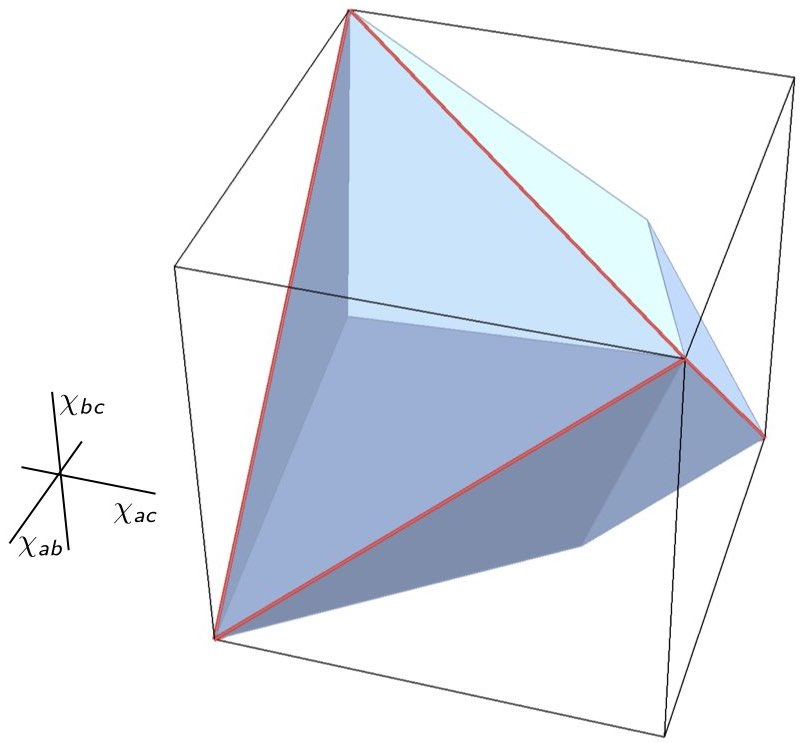
\includegraphics[width=4in]{polytope-spin1.jpeg} 
   \caption{Anti-correlation polyhedron for raffles simulating quantum correlations for spin-1 (cf.\ the classical tetrahedron in Figure \ref{tetrahedron}).}
   \label{polytope-spin1}
\end{figure}

To illustrate how this mapping works, consider the admissible raffle ($\beta$) introduced above. This raffle is represented by the point
\begin{equation}
(0, 0, 0, 0, 0, f^{\mathrm{vi}}_\beta, 0, f^{\mathrm{viii}}_\beta, 0, 0, 0, f^{\mathrm{xii}}_\beta, 0, 0)
\label{beta point simplex}
\end{equation}
of the 13D simplex, with $f^{\mathrm{vi}}_\beta = f^{\mathrm{viii}}_\beta = f^{\mathrm{viii}}_\beta = \sfrac13$ (see Eq.\ (\ref{spin 1 raffle beta})). We designed this raffle so that it is represented by the point $(-\sfrac12, -\sfrac12, -\sfrac12)$ of the anti-correlation polyhedron (see Eq.\ (\ref{raffle beta = -1/2^3})). We verify that $M$ correctly maps the point in Eq.\ (\ref{beta point simplex}) to the point in Eq.\ (\ref{raffle beta = -1/2^3}). For $\vec{f}_{\mathrm{adm}} = \vec{f}_\beta$, the mapping in Eq.\ (\ref{mapping spin 1 a}) reduces to:
\begin{equation}
\left. \begin{pmatrix}
\chi_{ab}\\[.3cm]
\chi_{ac}\\[.3cm]
\chi_{bc}
\end{pmatrix} \right|_{\vec{f}_\beta} = 
\left. \begin{pmatrix}
M_{ab}^{\mathrm{vi}} & \!\! M_{ab}^{\mathrm{viii}} \!\! & M_{ab}^{\mathrm{xii}} \\[.3cm]
M_{ac}^{\mathrm{vi}} & \!\! M_{ac}^{\mathrm{viii}} \!\! & M_{ac}^{\mathrm{xii}} \\[.3cm]
M_{bc}^{\mathrm{vi}} & \!\! M_{bc}^{\mathrm{viii}} \!\! & M_{bc}^{\mathrm{xii}}
 \end{pmatrix}
\!\! \begin{pmatrix}
f^{\mathrm{vi}} \\[.3cm]
f^{\mathrm{viii}} \\[.3cm]
f^{\mathrm{xii}}
\end{pmatrix} \right|_{\vec{f}_\beta}.
\label{mapping for raffle beta}
\end{equation}
Using  Eq.\ (\ref{components of M spin 1}) for the matrix elements of $M$ and setting these three components of $\vec{f}_\beta$ equal to $\sfrac13$, we confirm that
\begin{equation}
\left. \begin{pmatrix}
\chi_{ab}\\[.3cm]
\chi_{ac}\\[.3cm]
\chi_{bc}
\end{pmatrix} \right|_{\vec{f}_\beta}
=
 \begin{pmatrix}
0 & \!\!\!\! -\sfrac32 \!\!\!\! & 0 \\[.3cm]
-\sfrac32  & 0 & 0 \\[.3cm]
0 & 0 & -\sfrac32 
 \end{pmatrix}
 \begin{pmatrix}
\sfrac13 \\[.3cm]
\sfrac13\\[.3cm]
\sfrac13
\end{pmatrix} 
=
 \begin{pmatrix}
- \sfrac12 \\[.3cm]
- \sfrac12\\[.3cm]
- \sfrac12
\end{pmatrix}.
\label{mapping for raffle beta a}
\end{equation}

More generally, Eq.\ (\ref{mapping spin 1 a}) maps the 10D polytope of admissible raffles to the 3D anti-correlation polyhedron in Figure \ref{polytope-spin1}. This polyhedron is obtained by projecting the 40 vertices MathSage found for us and taking their convex hull. Once again using MathSage, we found that of the 40 points so projected, only 8 are vertices of the polyhedron. Four of them are the vertices of the tetrahedron in Figure \ref{tetrahedron}. The other four are the points $\left(\pm \sfrac12,\pm \sfrac 12,\pm \sfrac12\right)$ in which an odd number of minus signs occur. Raffle ($\beta$) is represented by the one with three minus signs (see Eqs.\ (\ref{raffle beta = -1/2^3}) and (\ref{mapping for raffle beta a})). To construct raffles represented by the three other points, we change the sign of the values $\pm 1$ for one of the three settings for all three ticket types in raffle ($\beta$). If this results in a ticket that is not among the fourteen tickets in Figure \ref{raffle-tickets-3set3out-i-xiv}, we simply switch the left and the right side of the ticket. The proportions of the tickets are kept the same. If we do this for setting $\hat{a}$, we get a new raffle ($\beta^{\prime}$) (with tickets of type (ii), (iv) and (xii)) for which
\begin{eqnarray}
\langle X^A_a X^B_b \rangle  \big|_{\vec{f}_{\beta^\prime}} = - \langle X^A_a X^B_b \rangle  \big|_{\vec{f}_\beta} = \sfrac12 \\[.2cm]
\langle X^A_a X^B_c \rangle  \big|_{\vec{f}_{\beta^\prime}} = - \langle X^A_a X^B_c \rangle  \big|_{\vec{f}_\beta} = \sfrac12 \\[.2cm]
\langle X^A_b X^B_c \rangle \big|_{\vec{f}_{\beta^\prime}}  = \langle X^A_b X^B_c \rangle  \big|_{\vec{f}_\beta} = - \sfrac12
\label{other vertices for spin 1}
\end{eqnarray}
If we do the same thing for setting $\hat{b}$, we get a second new raffle ($\beta^{\prime\prime}$) (with tickets of type (ii), (vi) and (x)), in which $\langle X^A_a X^B_c \rangle$ will be the same as in raffle ($\beta$) while the other two change sign. Finally, if do this for setting $\hat{c}$, we get a third new raffle ($\beta^{\prime\prime\prime}$) (with tickets of type (iv), (viii) and (x)), in which $\langle X^A_a X^B_b \rangle$ will be the same as in raffle ($\beta$) and the other two change sign. In the polyhedron in Figure \ref{polytope-spin1}, the raffles ($\beta^\prime$), ($\beta^{\prime\prime}$)  and  ($\beta^{\prime\prime\prime}$) are thus represented by the points $\left( \sfrac12, \sfrac 12,-\sfrac12\right)$, $\left(\sfrac12, - \sfrac 12, \sfrac12\right)$ and $\left( -\sfrac12, \sfrac 12,\sfrac12\right)$, respectively. 
%One sees in Figure \ref{polytope-spin1} that the four extra points the polyhedron of our raffles for the spin-1 case picks up compared to the tetrahedron for our raffles for the spin-$\frac12$ case lie at the center of each of the four parts into which the elliptope is divided by the tetrahedron. 


%SUBSUBSECTION 3.2.3
\subsubsection{Spin-$\frac32$} \label{2.2.3}


The flow chart in Figure \ref{flowchart} that we used to deal with raffles for the spin-1 case will also guide us in our analysis of raffles for the spin-$\frac32$ case. The number of tickets now jumps from $(3^3 +1)/2 = 14$ to $4^3/2 = 32$. We will only display a subset of these tickets (see Figures \ref{raffles-spin32-tickets-mu} and \ref{raffles-spin32-tickets-nu}). We numbered them using the same convention as before (cf.\ the tree structure in Figure \ref{raffle-tickets-3set2out-i-thru-iv} in Section \ref{1.4}). With 32 tickets, the number of vertices and facets to keep track of is starting to get unwieldy but the spin-$\frac32$ case is still tractable. And there are at least two good reasons for examining it in some detail: it is the simplest case in which cell symmetry calls for separate admissibility conditions; it nicely illustrates the difference between integer and half-integer spin cases in terms of the bound on the sum of the anti-correlation coefficients $\chi_{ab} + \chi_{bc} + \chi_{ac}$ (see Section \ref{1.6}, Eqs.\ (\ref{De Finetti half integer s})--(\ref{Mermin CHSH integer spin})).

\begin{figure}[ht]
 \centering
   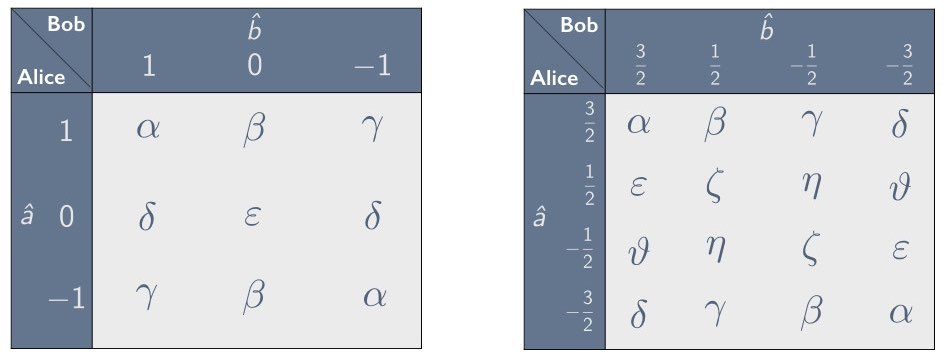
\includegraphics[width=4.5in]{symmetry-spin-1-32.jpeg} 
   \caption{Cell in the correlation arrays for the spin-1 and spin-$\frac32$ cases showing centrosymmetry.}
   \label{symmetry-spin-1-32}
\end{figure}

Figure \ref{symmetry-spin-1-32} shows a generic off-diagonal cell in the correlation array for two of our raffles, the one on the left for the spin-1 case, the one on the right for the spin-$\frac32$ case. As noted in the introduction to Section \ref{2}, the design of our raffles guarantees that these cells are centrosymmetric (see Eq.\ (\ref{raffle cell centro-symmetry})). Hence, 5 parameters (labeled $\alpha$ through $\varepsilon$) suffice to fix the 9 entries in the cell on the left and 8 parameters (labeled $\alpha$ through $\vartheta$) suffice to fix the 16 entries in the one on the right (these parameters have to satisfy the obvious requirement that the sum of all entries in a cell equals 1). 
%This means that Eq.\ (\ref{raffle cell centro-symmetry}) holds for any single-ticket or mixed raffle whatsoever. Centro-symmetry, in other words, does not require any restrictions on $\vec{f}$.

Requiring uniform marginals further reduces the number of parameters needed to determine the entries in the cells in Figure \ref{symmetry-spin-1-32}. The conditions ensuring uniform marginals in the spin-$\frac32$ case are a straightforward generalization of those in the spin-1 case (cf.\ Eq.\ (\ref{uniform marginals spin-1})):
\begin{equation}
\mathrm{Pr}\!\left({\textstyle{\frac32}} -\!\!{\textstyle{\frac32}} \Big|\hat{a}\hat{a}\!\right) \!\!  \Big|_{\!\vec{f}_{\mathrm{adm}}} \!\!\!
= \mathrm{Pr}\!\left({\textstyle{\frac12}} -\!\!{\textstyle{\frac12}} \Big|\hat{a}\hat{a}\!\right) \!\! \Big|_{\!\vec{f}_{\mathrm{adm}}} \!\!\!
= \mathrm{Pr}\!\left(-\!{\textstyle{\frac12}} \, {\textstyle{\frac12}} \Big|\hat{a}\hat{a}\!\right)  \!\! \Big|_{\!\vec{f}_{\mathrm{adm}}} \!\!\!
= \mathrm{Pr}\!\left(-\!{\textstyle{\frac32}} \, {\textstyle{\frac32}} \Big|\hat{a}\hat{a}\!\right) \!\! \Big|_{\!\vec{f}_{\mathrm{adm}}} \!\!\!
=  \frac14,
\label{uniform marginals spin-32}
\end{equation}
and similarly for the diagonal cells with settings $\hat{b}\,\hat{b}$ and $\hat{c}\,\hat{c}$. As in the spin-1 case, it suffices to impose one of these conditions for each diagonal cell:
\begin{equation}
\mathrm{Pr}\!\left({\textstyle{\frac32}} -\!\!{\textstyle{\frac32}} \Big|\hat{a}\,\hat{a}\right) \!  \Big|_{\vec{f}_{\mathrm{adm}}} \!\!
= \mathrm{Pr}\!\left({\textstyle{\frac32}} -\!\!{\textstyle{\frac32}} \Big|\hat{b}\,\hat{b}\right) \!  \Big|_{\vec{f}_{\mathrm{adm}}} \!\!
= \mathrm{Pr}\!\left({\textstyle{\frac32}} -\!\!{\textstyle{\frac32}} \Big|\hat{c}\,\hat{c}\right) \!  \Big|_{\vec{f}_{\mathrm{adm}}} \!\!
=  \frac14.
\label{uniform marginals spin-32 a}
\end{equation}

Once the conditions for uniform marginals have been imposed, the entries in the cell for the spin-1 case will satisfy
\begin{equation}
\alpha + \beta + \gamma = \alpha + \delta + \gamma = 2\beta + \varepsilon = \sfrac13.
\label{spin 1 relations parameters} 
\end{equation}
It follows that 
\begin{equation}
\gamma = \sfrac13 - \alpha - \beta, \quad \delta = \beta, \quad \varepsilon = \sfrac13 - 2\beta.
\label{spin 1 gamma delta epsilon}
\end{equation}
It thus only takes two independent parameters, $\alpha$ and $\beta$, to fix all entries in the cell. 

Note that this is still one more parameter than is needed to fix all entries in a cell in a correlation array for measurements on the singlet state of two particles of arbitrary (half-)integer spin $s$. The entries in those cells are fixed by (a highly non-linear function of) a single parameter, the angle $\varphi_{ab}$ between the measuring directions. It thus need not surprise us that, for $s \ge 1$, we can no longer perfectly simulate the quantum correlations (see Eq.\ (\ref{off diag cell quantum v raffle})).

Inserting the expressions for $\gamma$, $\delta$ and $\varepsilon$ in Eq.\ (\ref{spin 1 gamma delta epsilon}) in the cell for the spin-1 case in Figure \ref{symmetry-spin-1-32}, we see that this cell is now symmetric as well as centro-symmetric. As we noted in Section \ref{2.2.2}, requiring uniform marginals thus automatically ensures cell symmetry in the spin-1 case. 

In the spin-$\frac32$ case, this is no longer true. Instead of Eq.\ (\ref{spin 1 relations parameters}), the requirement of uniform marginals now gives 
\begin{equation}
\alpha + \beta + \gamma + \delta = \alpha + \varepsilon + \vartheta + \delta = \sfrac14,
\label{symmetry condition cell spin 32}
\end{equation}
from which it follows only that $\beta + \gamma = \varepsilon + \vartheta$. To ensure cell symmetry we need to impose an extra condition. We will set $\beta = \varepsilon$. Since Eq.\ (\ref{symmetry condition cell spin 32}) then entails $\gamma = \vartheta$, this suffices to make the cell on the right in Figure \ref{symmetry-spin-1-32} is symmetric. 

The condition $\beta = \varepsilon$ translates into
\begin{equation}
\left. \mathrm{Pr}\left({\textstyle{\frac32}} {\textstyle{\frac12}} \Big| \hat{a}\hat{b}\right)  \right|_{\vec{f}_{\mathrm{adm}}}
= \left. \mathrm{Pr}\left({\textstyle{\frac12}} {\textstyle{\frac32}} \Big| \hat{a}\hat{b}\right)  \right|_{\vec{f}_{\mathrm{adm}}}.
\label{symmetry condition spin 32} 
\end{equation}
We need three such conditions, one for each of the three off-diagonal cells in the correlation array (recall that the cell symmetry and the symmetry of the correlation array as a whole guarantee that cells on opposite sides of the diagonal are the same). The probabilities in these admissibility conditions are given by half the sum of the ticket fractions $f^{\mathrm{k}}_{\mathrm{adm}}$ for those tickets that have the relevant combination of outcomes (cf.\ Eqs.\ (\ref{chi for f spin 1/2 b})--(\ref{chi for f spin 1/2 ba})). Like the conditions for uniform marginals, these symmetry conditions thus take the form of linear constraints on the ticket fractions $f^\mathrm{k}$ (with k now running from i through xxxii). 

\begin{figure}[ht]
 \centering
   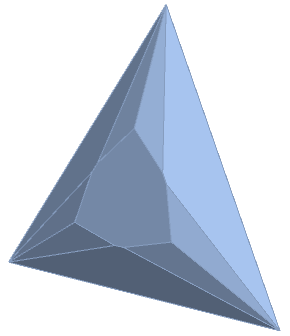
\includegraphics[width=3.5in]{SpinThreeHalfFace.png} 
   \caption{Facets of the anti-correlation polyhedron for spin-$\frac{3}{2}$. Imagine this figure `glued onto' the four facets of the classical tetrahedron in Figure \ref{tetrahedron}.}
   \label{SpinThreeHalfFace}
\end{figure}

For the spin-$\frac32$ case we have a total of 6 admissibility conditions, 3 to ensure uniform marginals, 3 to ensure cell symmetry. Since there are 32 different tickets, the polytope we start from is the 31D standard simplex in $\mathbb{R}^{32}$ (cf.\ the flow chart in Figure \ref{flowchart}). Upon imposing our 6 admissibility conditions, we arrive at a 25D polytope of admissible raffles in $\mathbb{R}^{32}$. With the help of Sagemath we find that this polytope has a total of 450 (!) vertices. We can map this polytope  in $\mathbb{R}^{32}$ to the 3D anti-correlation polyhedron using a $32 \, \times \, 3$ matrix $M$ with elements of the same form as those of the $14 \, \times \, 3$ matrix for raffles in the spin-1 case (see Eqs.\ (\ref{mapping spin 1 a})--(\ref{components of M spin 1}) and Table \ref{covariances for spin 1}). For our purposes we only need a subset of the 96 elements of this matrix (see Tables \ref{covariances for spin 3/2 raffle mu} and \ref{covariances for spin 3/2 raffle nu}). Applying the mapping given by the matrix $M$ to the 450 vertices of our 25D polytope and using Sagemath to determine which of the resulting 450 points are the vertices of its 3D image, we found a polyhedron in $\mathbb{R}^{3}$ with 40 vertices. We then used the program Mathematica to find the facets of this polyhedron and generate the picture in Figure \ref{SpinThreeHalfFace}. This picture shows the facets we need to ``glue onto" each of the four facets of the tetrahedron in Figure \ref{tetrahedron} to get the full anti-correlation polyhedron in this case.

The polyhedron for raffles (imperfectly) simulating the quantum correlations in the spin-$\frac32$ case picks up 36 extra vertices compared to the tetrahedron for raffles for the spin-$\frac12$ case, 9 for each facet of the tetrahedron. Figure \ref{SpinThreeHalfFace} shows those 9 extra vertices for one of these four facets, 6 of them in pairs that lie so close together that it may look as if there are only 6 rather than 9 points. All 9 vertices lie in the same plane. In the case of the facet of the tetrahedron closest to the point $(-1, -1, -1)$ of the non-signaling cube (see Figure \ref{tetrahedron}) this is the plane where the sum $\chi_{ab} + \chi_{ac} + \chi_{bc}$ has its minimum value. Eq.\ (\ref{Mermin CHSH half-integer spin}) in Section \ref{1.6} tells us that the minimum value of this quantity for $s = \sfrac32$ is
\begin{equation}
%\big( \chi_{ab} + \chi_{ac} + \chi_{bc} \big)_{{\mathrm{minimum \; for}}\; s \,= \, \sfrac32} 
 \frac{1}{8\sigma_{\sfrac32}^2} - \frac32 = \frac{1}{10} - \frac32 = -\frac75.
\end{equation}
where we used Eq.\ (\ref{SD for adm raffle 2}) to set $\sigma_{\sfrac32}^2 = \sfrac54$.

With a little help from the computer, we were able to construct raffles represented by these 9 vertices. Figures \ref{raffles-spin32-tickets-mu} and \ref{raffles-spin32-tickets-nu} show the mix of tickets for two of them, labeled ($\mu$) and ($\nu$). We obtain raffles represented by the other seven vertices by permutations of the outcomes for the three settings $\hat{a}$, $\hat{b}$ and $\hat{c}$ on all tickets in these two raffles (switching left and right sides of tickets if necessary). By changing the sign of the values for one of the settings on all tickets in these nine raffles (again switching sides of tickets if necessary), we can construct raffles for the 27 vertices obtained if the facets in Figure \ref{SpinThreeHalfFace} are ``glued on'' to the other three facets of the tetrahedron (this is the same procedure that we followed for the spin-1 case in Section \ref{2.2.2}).

\begin{figure}[ht]
 \centering
   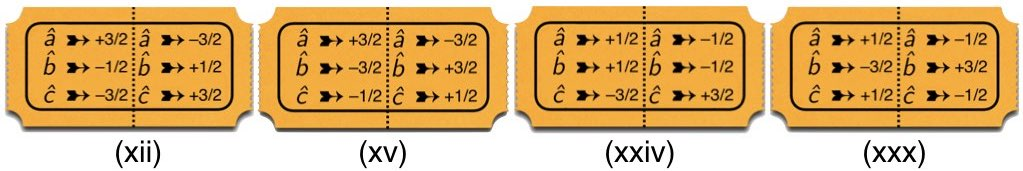
\includegraphics[width=4.5in]{raffles-spin32-tickets-mu.jpeg} 
   \caption{Admissible raffle ($\mu$) for the spin-$\frac32$ case with equal numbers of tickets of type (xii), (xv), (xxiv) and (xxx).}
    \label{raffles-spin32-tickets-mu}
\end{figure}

Consider Figure \ref{raffles-spin32-tickets-mu} for raffle ($\mu$) characterized by the vector
\begin{equation}
\vec{f}_\mu =  \frac14 \left( \vec{f}_{\mathrm{xii}} + \vec{f}_{\mathrm{xv}} + \vec{f}_{\mathrm{xxiv}} + \vec{f}_{\mathrm{xxx}} \right).
\label{vec spin 32 raffle mu}
\end{equation}

It is easy to see that this raffle yields uniform marginals: For all three settings, all four outcomes occur twice in every set of these four tickets. It is also easy to see that it will be represented by a point on the plane where $\chi_{ab} + \chi_{ac} + \chi_{bc}$ has its minimum value: On both sides of all four tickets, the sum of outcomes for the three settings is $\pm \sfrac12$ resulting in the minimum value of $\sfrac14$ of the expectation value of $(X^A_a + X^A_b + X^A_c)^2$ (cf.\ Section \ref{1.6}). To make sure that the off-diagonal cells in the correlation array for raffle ($\mu$) are symmetric, we check that Eq.\ (\ref{symmetry condition spin 32}) is satisfied, not just for the $\hat{a}\hat{b}$ cell but for the $\hat{a}\hat{c}$ and $\hat{b}\hat{c}$ cells as well. Since
\begin{equation}
\begin{array}{cc}
\mathrm{Pr}\!\left({\textstyle{\frac32}} {\textstyle{\frac12}} \Big| \hat{a}\hat{b}\right) \! \Big|_{\vec{f}_\mu} = {\textstyle{\frac12}} \, f^{\mathrm{xii}},  &
\mathrm{Pr}\!\left({\textstyle{\frac12}} {\textstyle{\frac32}} \Big| \hat{a}\hat{b}\right)  \! \Big|_{\vec{f}_\mu} = {\textstyle{\frac12}} \, f^{\mathrm{xxx}}, \\[.4cm]
 \mathrm{Pr}\!\left({\textstyle{\frac32}} {\textstyle{\frac12}} \Big| \hat{a}\hat{c}\right) \! \Big|_{\vec{f}_\mu}  = {\textstyle{\frac12}} \, f^{\mathrm{xv}}, &
\mathrm{Pr}\!\left({\textstyle{\frac12}} {\textstyle{\frac32}} \Big| \hat{a}\hat{c}\right)  \! \Big|_{\vec{f}_\mu}   = {\textstyle{\frac12}} \, f^{\mathrm{xxiv}}, \\[.4cm]
\mathrm{Pr}\!\left({\textstyle{\frac32}} {\textstyle{\frac12}} \Big| \hat{b}\hat{c}\right) \! \Big|_{\vec{f}_\mu}   = {\textstyle{\frac12}} \, f^{\mathrm{xxx}}, &
\mathrm{Pr}\!\left({\textstyle{\frac12}} {\textstyle{\frac32}} \Big| \hat{b}\hat{c}\right) \! \Big|_{\vec{f}_\mu}  = {\textstyle{\frac12}} \, f^{\mathrm{xxiv}},
\end{array}
\end{equation}
and all four ticket fractions are equal, these symmetry conditions are indeed satisfied.

Using Eq.\ (\ref{mapping spin 1 a}) for the mapping from ticket fractions of admissible raffles to triplets of allowed anti-correlation coefficients, we can find the components of $\vec{\chi}$ for raffle ($\mu$). In this case, Eq.\ (\ref{mapping spin 1 a}) reduces to
\begin{equation}
\left. \begin{pmatrix}
\chi_{ab}\\[.3cm]
\chi_{ac}\\[.3cm]
\chi_{bc}
\end{pmatrix} \right|_{\vec{f}_\mu}
= \left. \begin{pmatrix}
M_{ab}^{\mathrm{xii}} & M_{ab}^{\mathrm{xv}} & M_{ab}^{\mathrm{xxiv}} & M_{ab}^{\mathrm{xxx}} \\[.4cm]
M_{ac}^{\mathrm{xii}} & M_{ac}^{\mathrm{xv}} & M_{ac}^{\mathrm{xxiv}} &  M_{ac}^{\mathrm{xxx}} \\[.4cm]
M_{bc}^{\mathrm{xii}} & M_{bc}^{\mathrm{xv}} & M_{bc}^{\mathrm{xxiv}} &  M_{bc}^{\mathrm{xxx}}
 \end{pmatrix}
\!\! \begin{pmatrix}
f^{\mathrm{xii}} \\[.1cm]
f^{\mathrm{xv}} \\[.1cm]
f^{\mathrm{xxiv}} \\[.1cm]
f^{\mathrm{xxx}}
\end{pmatrix} \right|_{\vec{f}_\mu}. 
\label{mapping for raffle mu}
\end{equation}
The ticket fractions are all equal to $\sfrac14$. The elements of the matrix $M$ are given by
\begin{equation}
M^{\mathrm{k}}_{ab} = -\frac{1}{\sigma_{s = \sfrac32}^2} \langle X^A_a X^B_b \rangle, \quad \mathrm{with \; k  =  i \, \ldots \, xxxii},  
\end{equation}
and similar expressions with $ab$ replaced by $ac$ or $bc$ (cf.\ Eq.\ (\ref{M_ab^i spin-1})). These matrix elements are given by $- 1/\sigma_{s = \sfrac32}^2 = -\sfrac45$ times the relevant entries in Table \ref{covariances for spin 3/2 raffle mu}. 

\begin{table}[ht]
\centering
\begin{tabular}{|c||c|c|c|}
\hline
\Big. ticket & $\langle X^A_a X^B_b \rangle$ & $\langle X^A_a X^B_c\rangle$  &  $\langle X^A_b X^B_c \rangle$\\
\hline
\Big. (xii)$_{[\frac32-\frac12-\frac32]}$  & $\sfrac34$ & $\sfrac94$ & $-\sfrac34$ \\[.2cm]
(xv)$_{[\frac32-\frac32-\frac12]}$ & $\sfrac94$ & $\sfrac34$ & $-\sfrac34$ \\[.2cm]
(xxiv)$_{[\frac12\frac12-\frac32]}$ & $-\sfrac14$ & $\sfrac34$ & $\sfrac34$ \\[.2cm]
(xxx)$_{[\frac12-\frac32\frac12]}$ & $\sfrac34$ & $-\sfrac14$ & $\sfrac34$ \\[.2cm]
 \hline
\end{tabular}
\caption{Covariances for single-ticket raffles for the four ticket types in admissible raffle ($\mu$) in Figure \ref{raffles-spin32-tickets-mu}
%The subscript on each ticket number gives the values for the settings $\hat{a}$, $\hat{b}$ and $\hat{c}$ on the left side of a ticket of that type 
(cf.\ Table \ref{covariances for spin 1}).}
\label{covariances for spin 3/2 raffle mu}
\end{table} 

For the components of $\vec{\chi}$ for raffle ($\mu$) we then find:
\begin{equation}
\left. \begin{pmatrix}
\chi_{ab}\\[.3cm]
\chi_{ac}\\[.3cm]
\chi_{bc}
\end{pmatrix} \right|_{\vec{f}_\mu}
= 
\begin{pmatrix}
-\sfrac35 & -\sfrac95 & \sfrac15 & -\sfrac35 \\[.3cm]
-\sfrac95 & -\sfrac35 & -\sfrac35 & \sfrac15 \\[.3cm]
\sfrac35 & \sfrac35 & -\sfrac35 & -\sfrac35 
\end{pmatrix}
\begin{pmatrix}
\sfrac14 \\[.1cm]
\sfrac14 \\[.1cm]
\sfrac14 \\[.1cm]
\sfrac14
\end{pmatrix}
= 
\begin{pmatrix}
-\sfrac{7}{10} \\[.3cm]
-\sfrac{7}{10} \\[.3cm]
0
\end{pmatrix},
\end{equation}
which confirms that $\chi_{ab} + \chi_{ac} + \chi_{bc} =- \sfrac75$, as it should be given the way we constructed this raffle. Raffle ($\mu$) is represented by one of the 9 vertices in the plane of the polyhedron where $\chi_{ab} + \chi_{ac} + \chi_{bc}$ has its minimum value. Through suitable permutation of the outcomes for settings $\hat{a}$,  $\hat{b}$ and  $\hat{c}$, we can create raffles similar to raffle ($\mu$) represented by two other vertices in that same plane: $(0, -\sfrac{7}{10}, -\sfrac{7}{10})$ and $(-\sfrac{7}{10}, 0, -\sfrac{7}{10})$.

%Now consider a raffle ($\mu^\prime$) obtained by replacing all values for $\hat{a}$ on both sides of the four ticket types in raffle ($\mu$) by the values for $\hat{b}$, the values for $\hat{b}$ by those for $\hat{c}$ and the values for $\hat{c}$ by those for $\hat{a}$. The values for $(\chi_{ab}, \chi_{ac}, \chi_{bc})$ for this new raffle ($\mu^\prime$) will be given by the values for $(\chi_{bc}, \chi_{ba} = \chi_{ab}, \chi_{ca} = \chi_{ac})$ for raffle ($\mu$). Raffle ($\mu$) will thus be represented by the point $(0, -\sfrac{7}{10}, -\sfrac{7}{10})$ on the same plane as the point representing raffle ($\mu$). A similar permutation produces a raffle ($\mu^{\prime\prime}$) represented by the point $(-\sfrac{7}{10}, 0, -\sfrac{7}{10})$ on that plane.   

\begin{figure}[ht]
 \centering
   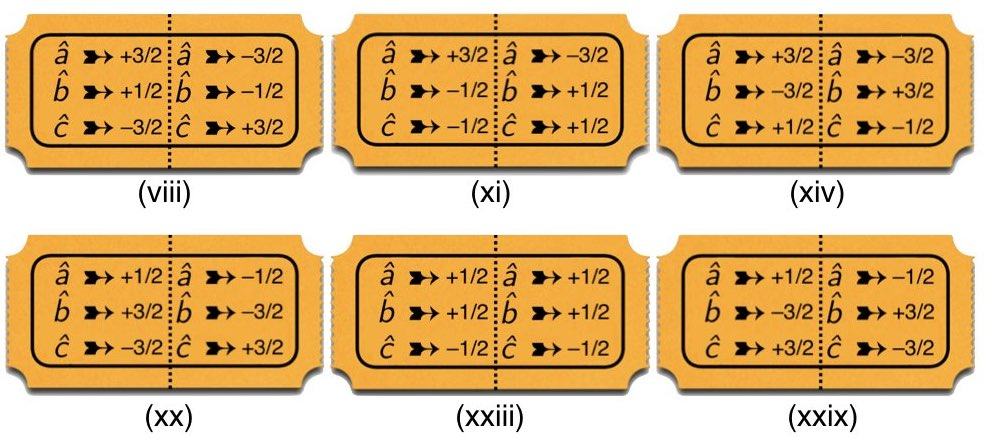
\includegraphics[width=4.5in]{raffles-spin32-tickets-nu.jpeg} 
   \caption{Admissible raffle ($\nu$) for the spin-$\frac32$ case: a basket with equal numbers of tickets of type (viii), (xi), (xiv), (xx), (xxiii) and (xxix).}
    \label{raffles-spin32-tickets-nu}
\end{figure}

Figure \ref{raffles-spin32-tickets-nu} shows the tickets for a raffle represented by one of the remaining six points in the plane where $\chi_{ab} + \chi_{ac} + \chi_{bc} = -\sfrac75$. This raffle is represented by the vector 
\begin{equation}
\vec{f}_\nu =  \frac16 \left( \vec{f}_{\mathrm{viii}} + \vec{f}_{\mathrm{xi}} + \vec{f}_{\mathrm{xiv}} + \vec{f}_{\mathrm{xx}} + \vec{f}_{\mathrm{xxiii}} + \vec{f}_{\mathrm{xxix}} \right),
\label{vec spin 32 raffle nu}
\end{equation}
As with raffle ($\mu$), the outcomes of both sides of all tickets add up to $\pm \sfrac12$ and both sets of admissibility conditions (uniform marginals and cell symmetry) are met. These last two properties can be verified the same way as in the case of raffle ($\mu$). 

\begin{table}[ht]
\centering
\begin{tabular}{|c||c|c|c|}
\hline
\Big. ticket & $\langle X^A_a X^B_b \rangle$ & $\langle X^A_a X^B_c\rangle$  &  $\langle X^A_b X^B_c \rangle$\\
\hline
\Big. (viii)$_{[\frac32\frac12-\frac32]}$ & $-\sfrac34$ & $\sfrac94$ & $\sfrac34$ \\[.2cm]
(xi)$_{[\frac32-\frac12-\frac12]}$ & $\sfrac34$ & $\sfrac34$ & $-\sfrac14$ \\[.2cm]
(xiv)$_{[\frac32-\frac32\frac12]}$ & $\sfrac94$ & $-\sfrac34$ & $\sfrac34$ \\[.2cm]
(xx)$_{[\frac12\frac32-\frac32]}$ & $-\sfrac34$ & $\sfrac34$ & $\sfrac94$ \\[.2cm]
(xxiii)$_{[\frac12\frac12-\frac12]}$ & $-\sfrac14$ & $\sfrac14$ & $\sfrac14$ \\[.2cm]
(xxix)$_{[\frac12-\frac32\frac32]}$ & $\sfrac34$ & $-\sfrac34$ & $\sfrac94$ \\[.2cm]
 \hline
\end{tabular}
\caption{Covariances for single-ticket raffles for the six ticket type in admissible raffle ($\nu$) in Figure \ref{raffles-spin32-tickets-nu} (cf.\ Table \ref{covariances for spin 3/2 raffle mu}).}
\label{covariances for spin 3/2 raffle nu}
\end{table} 

To find the components of $\vec{\chi}$ for this raffle, we once again use Eq.\ (\ref{mapping spin 1 a}), which in this case reduces to:
\begin{equation}
\left. \begin{pmatrix}
\chi_{ab}\\[.3cm]
\chi_{ac}\\[.3cm]
\chi_{bc}
\end{pmatrix} \right|_{\vec{f}_\nu}
= \left. \begin{pmatrix}
M_{ab}^{\mathrm{viii}} & M_{ab}^{\mathrm{xi}} & M_{ab}^{\mathrm{xiv}} & M_{ab}^{\mathrm{xx}} & M_{ab}^{\mathrm{xxiii}} & M_{ab}^{\mathrm{xxix}} \\[.3cm]
M_{ac}^{\mathrm{viii}} & M_{ac}^{\mathrm{xi}} & M_{ac}^{\mathrm{xiv}} & M_{ab}^{\mathrm{xx}} & M_{ab}^{\mathrm{xxiii}} & M_{ac}^{\mathrm{xxix}} \\[.3cm]
M_{bc}^{\mathrm{viii}} & M_{bc}^{\mathrm{xi}} & M_{bc}^{\mathrm{xiv}} & M_{ab}^{\mathrm{xx}} & M_{ab}^{\mathrm{xxiii}} & M_{bc}^{\mathrm{xxix}}
 \end{pmatrix}
\!\! \begin{pmatrix}
f^{\mathrm{viii}} \\
f^{\mathrm{xi}} \\
f^{\mathrm{xiv}} \\
f^{\mathrm{xx}} \\
f^{\mathrm{xxiii}} \\
f^{\mathrm{xxix}}
\end{pmatrix} \right|_{\vec{f}_\nu}.
\label{mapping for raffle nu}
\end{equation}
Evaluating the relevant elements of the matrix $M$ with the help of Table \ref{covariances for spin 3/2 raffle nu} and setting all ticket fractions equal to $\sfrac16$, we arrive at
\begin{equation}
\left. \begin{pmatrix}
\chi_{ab}\\[.3cm]
\chi_{ac}\\[.3cm]
\chi_{bc}
\end{pmatrix} \right|_{\vec{f}_\nu}
= \begin{pmatrix}
\sfrac35 & -\sfrac35 & -\sfrac95 & \sfrac35 & \sfrac15 & -\sfrac35 \\[.3cm]
-\sfrac95 & -\sfrac35 & \sfrac35 & -\sfrac35 & -\sfrac15 & \sfrac35  \\[.3cm]
-\sfrac35 & \sfrac15 & -\sfrac35 & -\sfrac95 & -\sfrac15 & -\sfrac95 
 \end{pmatrix}
\!\! \begin{pmatrix}
\sfrac16 \\
\sfrac16 \\
\sfrac16 \\
\sfrac16 \\
\sfrac16 \\
\sfrac16
\end{pmatrix}
= \begin{pmatrix}
-\sfrac{4}{15} \\[.3cm]
-\sfrac{5}{15}\\[.3cm]
-\sfrac{12}{15}
\end{pmatrix}.
\label{mapping for raffle nu a}
\end{equation}
Note that, once again, $\chi_{ab} + \chi_{ac} + \chi_{bc} =- \sfrac75$, as it should be given the way we constructed this raffle. Through suitable permutation of the outcomes for settings $\hat{a}$,  $\hat{b}$ and  $\hat{c}$, we can create raffles similar to raffle ($\nu$) represented by five other vertices of the facet of the anti-correlation polyhedron where $\chi_{ab} + \chi_{ac} + \chi_{bc} =- \sfrac75$. Since $\sfrac{4}{15}$ and $\sfrac13$ only differ by $\sfrac{1}{15}$, these six vertices can naturally be grouped into three pairs of neighboring points that are hard to tell apart in Figure \ref{SpinThreeHalfFace}:
\begin{equation}
\begin{array}{c}
\big\{ \left( -\sfrac{4}{15}, -\sfrac{1}{3}, -\sfrac{4}{5} \right), \left( -\sfrac{1}{3}, -\sfrac{4}{15}, -\sfrac{4}{5} \right) \big\}, \\[.3 cm]
\big\{ \left( -\sfrac{4}{5}, -\sfrac{4}{15}, -\sfrac{1}{3} \right), \left( -\sfrac{4}{5}, -\sfrac{1}{3}, -\sfrac{4}{15} \right) \big\},  \\[.3 cm]
\big\{ \left( -\sfrac{4}{15}, -\sfrac{4}{5}, -\sfrac{1}{3} \right),  \left( -\sfrac{1}{3}, -\sfrac{4}{5}, -\sfrac{4}{15} \right) \big\}.
\end{array}
\label{six vertices raffle nu}
\end{equation} 

The analysis of raffles ($\mu$) and ($\nu$) allowed us to understand the structure of the facets in Figure \ref{SpinThreeHalfFace} 
%of the polyhedron representing admissible raffles meant to simulate the quantum correlations for measurements on two spin-$\frac32$ particles entangled in the singlet state. 
in full detail.
For higher-spin cases, this becomes impractical. In the next subsection, we will therefore explore alternative methods for dealing with these higher-spin cases.
